
\section{KIDs systematic effect : non linearity}
\label{sec:KID-systematics}

In view of future uses of KIDs in a spatial environment, it is necessary to demonstrate the capabilities and the suitability of KIDs arrays in a space mission. In this section we will adress one of the systematic effects that need to be taken into account during the design of futur generation detector arrays for space applications, which is the KIDs non-linearity. Here we describe the simulation method used to study the KIDs non-linearity, then we will study the response of a KID to different sources and finally we will do realistic simulations in the context of a space mission.

\subsection{Simulations}

The KID linearity has been demonstrated, over a large power range, in laboratory
under realistic conditions as shown in Fig.~\ref{fig:KID-lin}. As we can see, at
300K the response of the KID is still under a linear regime.

%% \begin{figure}[h]
%% \center
%% 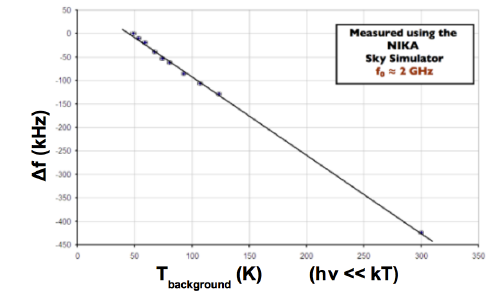
\includegraphics[clip, angle=0, width=\columnwidth]{Figures/KID-linearity-Monfardini2014.png}
%% \caption{KID linearity demonstrated in laboratory under realistic conditions. The plot shows the frequency shift of the resonance as a function of the optical background temperature (K). Solid line : linear fit of the experimental points. Credits : \citet{2014JLTP..176..787M}.}
%% \label{KID-lin}
%% \end{figure}

In this section we will adress the KID non-linearity by doing simulations that consist in modelling the response of a KID to a scan of a bright source, then to reconstruct the signal with the two methods described in Sec.~\ref{sec:signal}. This bright source is typically a planet, considered point like 

\begin{figure}[h]
\center
%\includegraphics[clip, angle=0, width=\columnwidth]{Figures/planets.eps}
%\caption{Comparison of the incoming flux (in black) with the signals
%  reconstructed by using \rf\ (in blue) and \cf\ (in red). In the top pannel and
%  bottom pannels, the incoming fluxes are respectively $10^{4}$ Hz and $10^{5}$
%  Hz. \todo{add a plot of the circle next to this one to show the excursion of $(\I,\Q)$}}
\includegraphics[clip, angle=0, width=\columnwidth]{Figures/planet_profiles.eps}
\caption{Comparison of the incoming flux (in black) with the reconstructed flux
  for various input fluxes and with the \rf\ and \cf method. Fluxes are
  unrealistically large on purpose for illustration. Non linearity
  appears with the distortion of the input gaussian profile in the case of the
  \rf\ method whereas \cf\ remains linear on the same flux scale \todo{rephrase
    better and address the 3 vs 5 points per FWHM}.}
\label{fig:planets}
\end{figure}

\begin{figure}[h]
\center
\includegraphics[clip, angle=0, width=\columnwidth]{Figures/resonance.eps}
\caption{Simulation of a resonance in the $I-Q$ plane, for incoming fluxes equal to $10^{4}$ (in red) and $10^{5}$ (in black) Hz.}
\label{fig:resonance}
\end{figure}

Fig.\ref{fig:planets} represents the reconstructed signal with different incoming flux. 
We observe that at higher flux the signal reconstructed by \rf\ is attenuated in comparison to the incident flux and the signal reconstructed by \cf . Fig. \ref{fig:resonance} represents the corresponding sweep of $I-Q$ around the resonance.

In order to derive the KID non-linearity, we do a gaussian fit of the outcoming signal, to calculate its flux. Then we plot the incoming flux as a function of the outcoming flux and fit this function by a polynomial :

\begin{equation}
\phi_{out}^{Rf,Cf} = g \delta P_{opt} + \varepsilon \delta (P_{opt})^2 +c_{0},
\label{eq:fit-nl}
\end{equation}

with : 
\begin{equation}
\phi_{out}^{Rf,Cf} \propto \delta f_{0} \sim \delta P_{opt}.\\
\end{equation}

$c_{0}$ is a constant and \eps\ is the non-linearity coefficient. \\

Many experiments such as MAXIPOL \citep{2007ApJ...665...42J}, EBEX
\citep{2010SPIE.7741E..1CR}, POLARBEAR \citep{2017JCAP...05..008T}, \nika2
\citep{2017A&A...599A..34R}, use half-wave plates (HWPs) to improve the
sensitivity in polarization measurments by naturally rejecting atmospheric
noise, and to reconstruct the three Stokes parameters : $I$ , $Q$ and $U$
. However, the rotation of the HWP induces a strong additional parasitic signal
that is highly peaked at harmonics of the HWP rotation frequency. This parasitic
signal is due to imperfections of the HWP that modulate the background signal,
it was observed by experiments like \nika2 \citep{2017A&A...599A..34R}, EBEX
\citep{2010SPIE.7741E..1CR} and MAXIPOL \citep{2007ApJ...665...42J}.  The power
spectrum illustrated in Fig.~\ref{fig:hwp_power_spectrum} shows this additionnal
noise that is two to three order of magnitude above the noise level, making it
one of the strongest noise contributor in polarization observations. Experiment
like \nika\ corrected this effect by fitting it by a sum of harmonics of the HWP
rotation frequency and subtracting it fom the TOIs. As you can see in
Fig.~\ref{fig:hwp_power_spectrum}, the parasitic signal was corrected and its
amplitude was reduced to noise level, but the residuals of this signal could
still induce non-linearity in the measurement. In this paper we will study this
systematic effect and see if it biases the measurment of a KID. To do so, we
simulate this signal by modelling it as a Fourier series of the harmonics of the
HWP rotation frequency :

\begin{equation}
HWP(t) = \sum_{n=1}^{6} A_{n} \cos nwt + B_{n} \sin nwt , 
\label{eq:hwp-template}
\end{equation}

with n the number of harmonics of the HWP rotation frequency.

\begin{figure}[h]
\center
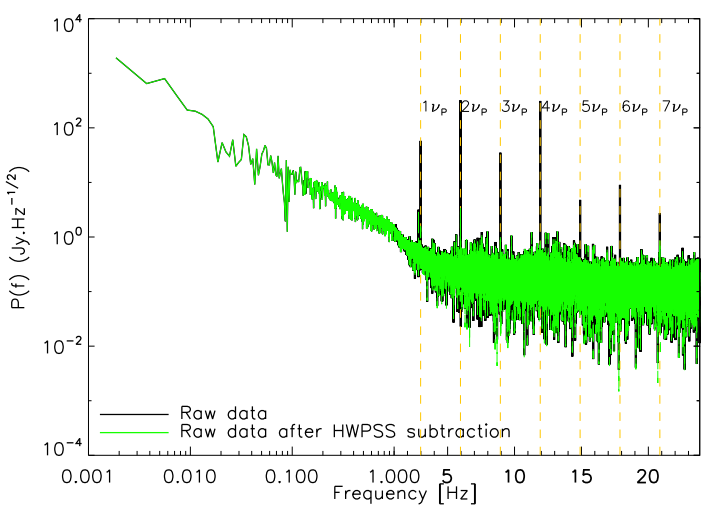
\includegraphics[clip, angle=0, width=\columnwidth]{Figures/hwp_power_spectrum.png}
\caption{Power spectrum of an observation of Orion OMC-1 for one KID. The observations were done with \nika . Black and green lines represent respectively the raw data and the raw data after subtraction of the HWP parasitic signal. Credits : \citet{2017A&A...599A..34R} }
\label{fig:hwp_power_spectrum}
\end{figure}

In the following paragraph, we will use the model described by Eq.~(\ref{eq:fit-nl}) to study the KID non-linearity when it is exposed to a planet and a HWP template.

\subsection{Results}

We do several simulations following the method described earlier. In these simulations we do a scanning strategy that ensures that the scanning speed is such that the number of points per beam is between 3 and 5 to respect the Nyquist criteria. For all simulations we model a planet by simulating a gaussian with amplitudes between 10 and 40 Jy. To see the evolution of the KID non-linearity as a function of the HWP signal, we add the HWP template that we modelled to the signal of the source and then we subtract it from the output signals.\\


Fig \ref{fig:diff-rf-cf} shows the results of these simulations by plotting the difference between the input and output signals. We can see on the top plot that for the worst case (incoming signal : planet, dipole and HWP), for both \rf\ and \cf\ the signals were well reconstructed as the difference between the input and output signal is less than $ 1 \%$. For \rf\ this difference derives more and is bigger than for \cf\, so using \cf\ is better because it adds less non-linearites than \rf . In addition, the plot shows that there is less non-linearities if you do the scan with more points per beam. As we can see in the bottom plot which represents the difference between the output and input signals but for different sources, the addition of the HWP template slightly adds some non-linearity to the measurment. In fact, at 40 Jy, there is a difference of less than $1 \%$ between the output signal of a planet only and a planet plus a HWP template meaning that adding a HWP template to the source do not bias the signal.

\begin{figure}[h]
  \includegraphics[clip, angle=0, width=\columnwidth]{Figures/diff-rf-cf.eps}
  \caption{Top : Difference between the output and input signals as a function of the incoming Planet flux (Jy). The incoming signal corresponds to a planet, a dipole and the HWP template. Blue and red lines correspond to signals reconstructed with \rf\ and \cf. Solid lines : scan with 5 points per beam. Dashed lines : scan with 3 points per beam.
    Bottom : Difference between the output and input signals as a function of the incoming Planet flux (Jy). The green, blue, red and turquoise lines correspond respectively to incoming signals consisting of a planet, planet and dipole, planet and HWP, planet and HWP and dipole. The signals were reconstructed with \rf. }
  \label{fig:diff-rf-cf}
\end{figure}

\begin{figure}[h]
  \includegraphics[clip, angle=0, width=\columnwidth]{Figures/diff-rf-cf-10-200jy-2.eps}
  \caption{same mais de 10 a 200 Jy}
  \label{fig:diff-rf-cf}
\end{figure}


For all simulations we computed the non-linearity coefficient \epsDET\ from Eq.~(\ref{eq:fit-nl}) in Tab.~\ref{tab:eps}. For \rf\ and \cf , \epsDET\ are respectively in the range of ($10^{-6}$-$10^{-5}$) and ($10^{-8}$-$10^{-7}$). Plus, for both methods the non-linearity coefficient is smaller when we scan the planet with 5 points per beam. In Sec.~\ref{sec:cmb} we saw that the non-linear coefficient related to the detector \epsDET has to be lower than \epsCMB. If we compare Tab.~\ref{tab:eps} and Tab.~\ref{tab:eps-lkg} we can see that we meet the conditions to reach $B$ modes at a tensor-to-scalar ratio of 0.001 for signals reconstructed with \cf , but we are at the limit with \rf .\\

\begin{table}
\tiny
\begin{tabular}{|c|c|c|c|c|}
	\hline
	    & \multicolumn{2}{|c|}{\rf} & \multicolumn{2}{|c|}{\cf} \\
	\hline
	    & $\frac{3pts}{beam}$ & $\frac{5pts}{beam}$ & $\frac{3pts}{beam}$ & $\frac{5pts}{beam}$ \\
	    \hline
	    $\varepsilon_{Pl}$ & -9.09 x $10^{-6}$ & -8.95 x $10^{-6}$ & 3.87 x $10^{-8}$ & 3.81 x $10^{-8}$ \\ 
	    \hline
	    $\varepsilon_{Pl+dip}$ & -9.34 x $10^{-6}$ & -9.20 x $10^{-6}$ & 3.70 x $10^{-8}$ & 3.64 x $10^{-8}$ \\
	    \hline
	    $\varepsilon_{Pl+hwp}$ & -1.27 x $10^{-5}$ & -1.25 x $10^{-5}$ & -4.13 x $10^{-7}$ & -4.00 x $10^{-7}$ \\
	\hline
	$\varepsilon_{Pl+hwp+dip}$ & -1.30 x $10^{-5}$ & -1.28 x $10^{-5}$ & -4.06 x $10^{-7}$ & 4.00 x $10^{-7}$ \\
	\hline
\end{tabular}
\caption{Non-linearity coefficients $\varepsilon$. The incoming flux corresponds to a planet (40 Jy).}
\label{tab:eps}
\end{table}

\begin{table}
\tiny
\begin{tabular}{|c|c|c|c|c|}
	\hline
	    & \multicolumn{2}{|c|}{\rf} & \multicolumn{2}{|c|}{\cf} \\
	\hline
	    & $\frac{3pts}{beam}$ & $\frac{5pts}{beam}$ & $\frac{3pts}{beam}$ & $\frac{5pts}{beam}$ \\
	    \hline
	    $\varepsilon_{Pl}$ & -3.13 x $10^{-5}$ & -3.08 x $10^{-5}$ & 1.23 x $10^{-7}$ & 1.22 x $10^{-7}$ \\ 
	    \hline
	    $\varepsilon_{Pl+hwp}$ & -1.97 x $10^{-5}$ & -1.94 x $10^{-5}$ & -6.02 x $10^{-7}$ & -5.95 x $10^{-7}$ \\
	\hline
\end{tabular}
\caption{same mmais seulement avec pl et pl+hwp}
\label{tab:eps}
\end{table}

In conclusion, in this part, we studied the KIDs non-linearity by simulating the detector response to a planet (10-40 Jy) and a HWP template. To reconstruct the signal we used two methods : \rf\ and \cf . Both methods could reconstruct the signal with a difference between the output and input signals of less than $1 \%$. We have seen that the non-lineaity coefficients derived while using \cf\  ($\sim 10^{-8} - 10^{-7} $)  are smaller than the ones with \rf   ($\sim 10^{-6} - 10^{-5} $). So even if \rf\ can already reconstruct the signal very well, by using \cf\ we add less non-linearities than by using \rf\.  Plus, adding a HWP template to an incoming signal consisting of a planet only slightly adds non-linearity to the signal and so does not bias the measurement. We have shown that this systematic effect depends on the flux of the incoming source and on the scanning speed, and that the results with a planet are positives. So in the next paragraph, we will study realistic simulations by using a scanning strategy typical of a satellite to scan the Galaxy which is more complex than a planet and to ensure that its signal can be reconstructed with \rf\ and \cf .
		
\subsubsection{Scanning strategy : EPIC, Planck}
A key factor in the design of space experiments is the scanning strategy of the instrument, as it conditions all the observations. Here, we present different simulations of scanning strategies such as the ones used in EPIC \citep{2009arXiv0906.1188B}, and Planck \citep{2005A&A...430..363D}. \\

Fig.~\ref{fig:satellite} shows a representation of a satellite, where $\alpha$ is the angle between the spin axis and the precession axis, and $\beta$ is the angle between the optical and spin axis of the satellite.
For EPIC scanning strategy, the optical axis of the telescope is inclined by $\beta$=55$\degree$ with respect to the spin axis The spin axis is inclined by $\alpha$=45$\degree$ from the precession axis and it precesses around the Sun-Earth axis every hour.
Planck scans large circles on the sky with a 85$\degree$ angle between the optical axis and the spin axis. The precession angle is 7$\degree$.

\begin{figure}[h]
  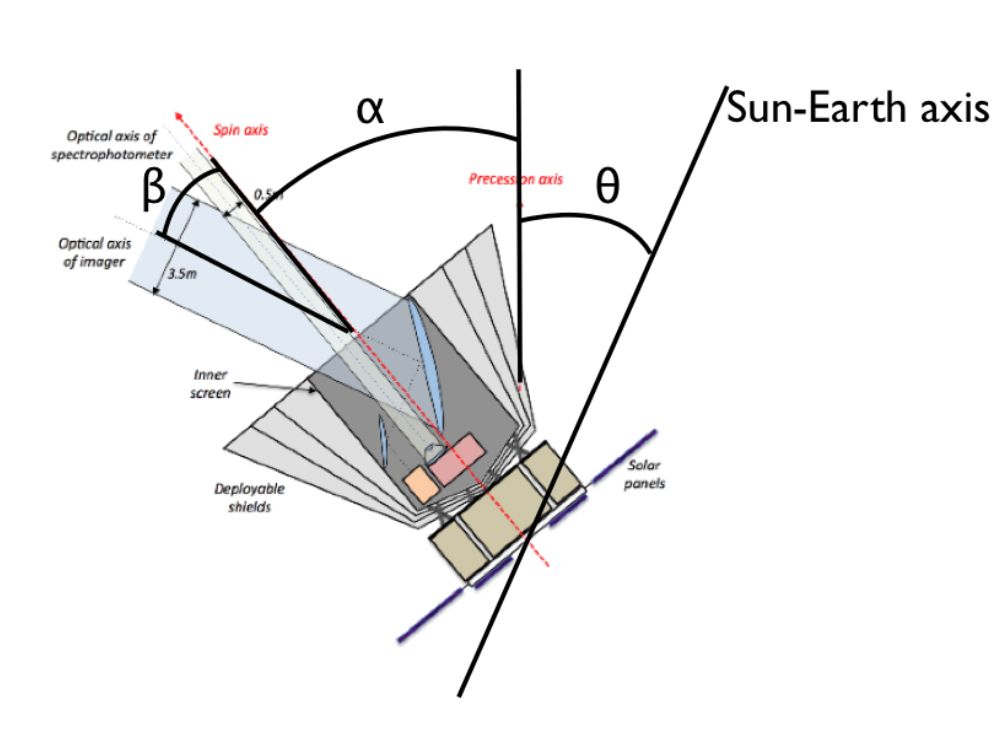
\includegraphics[clip,angle=0,width=\columnwidth]{Figures/schema_satellite.png}
  \caption{Schematic view of a satellite}
  \label{fig:satellite}
\end{figure}

The two scanning strategies are represented in Fig.~\ref{fig:strat-polsat-Planck}.

\begin{figure}[h]
  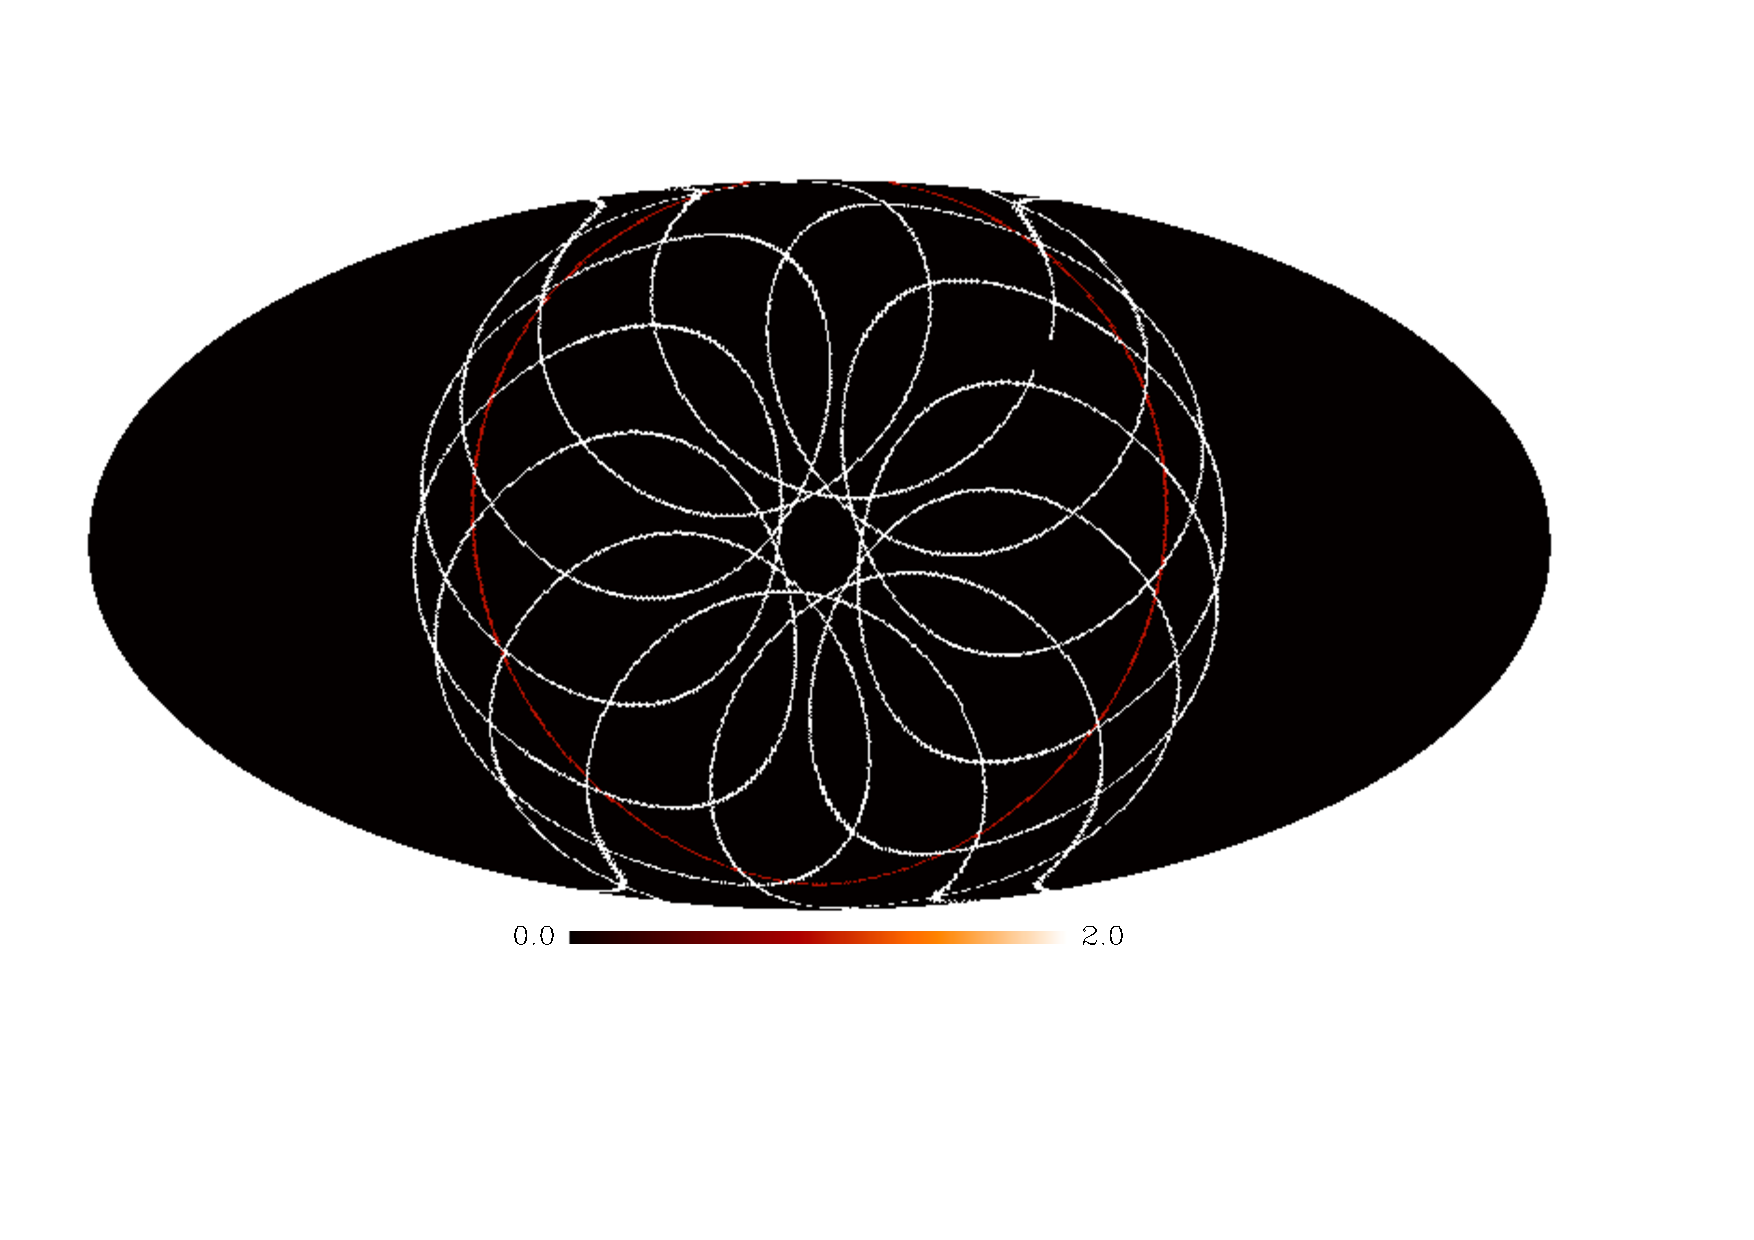
\includegraphics[clip,angle=0,width=\columnwidth]{Figures/plot_mollweide.pdf}
  \caption{White : representation of EPIC scanning strategy. Red : representation of Planck scanning strategy }
  \label{fig:strat-polsat-Planck}
\end{figure}

In the next paragraph we will do a more realistic simulation by using these scanning strategies to scan a map of the Galaxy (REF) and the cosmological dipole.

\subsubsection{Results}

Here we scan a map of the Galaxy with the two pointing strategies described earlier. In addition to the Galaxy, there is another signal that we have to take into account which is the CMB dipole. The CMB dipole is a smooth gradient in the CMB temperature accross the sky. It is the result of the motion of the local group of galaxies with respect to the reference framed defined by the CMB. The CMB dipole amplitude is $\Delta T = 3.365 \pm 0.027$ mK and directed toward $(l,b) = (264.4 \degree \pm 0.3 \degree , 48.4 \degree \pm 0.5 \degree)$ in galactic coordinates \citep{2015IJMPD..2430004B}. Like in the precedent simulations we add the template of HWP that we subtract after the signal goes through the KID model.

We have seen previously that to be in a linear regime, constraints had to be put on the scanning strategy, especially on the scanning speed, and on the incoming flux. Here the scanning strategy that we use ensure that we respect the Nyquist criteria, by having a number of points per beam between 3 and 5. Plus, we can see in Fig.~\ref{fig:histo-gal-dip}, that the flux of the Galaxy and Dipole does not go higher than 20 Jy and that the two methods \rf\ and \cf\ can reconstruct it. So considering the scanning strategy and the incoming flux, we can conclude that this simulation is in the regime where \eps\ is ranged between $10^{-6} - 10^{-5}$ for \rf , and $10^{-8} - 10^{-7}$ for \cf . 

\begin{figure}[h]
  \includegraphics[clip,angle=0,width=\columnwidth]{Figures/histo_gal_dip_epic.eps}
  \caption{Top : Histogram of the flux of the Galaxy and dipole in Jy. Bottom : Representation of the incoming flux (Galaxy, Dipole and HWP in black) and its reconstruction using \rf\ (blue) and \cf\ (red), in Jy. The Galaxy was scanned using Planck scanning strategy.}
  \label{fig:histo-gal-dip}
\end{figure}

\begin{figure}[h]
  \includegraphics[clip,angle=0,width=\columnwidth]{Figures/histo_gal_dip_planck.eps}
  \caption{Top : Histogram of the flux of the Galaxy and dipole in Jy. Bottom : Representation of the incoming flux (Galaxy, Dipole and HWP in black) and its reconstruction using \rf\ (blue) and \cf\ (red), in Jy. The Galaxy was scanned using Planck scanning strategy.}
  \label{fig:histo-gal-dip}
\end{figure}



To conclude, KIDs are a promising new type of technology. Here, we studied the KID response to several sources such as a planet, the CMB dipole and a signal from a HWP. We observed that we needed to put constraints on the scanning strategy, consequently we did more realistic simulations by scanning a map of the Galaxy and the dipole, by using the scanning strategy of a satellite (EPIC, Planck). In all the simulations, we have seen that the response of a KID is linear. In fact, the non-linearity coefficients that we derived are low (\eps $\simeq 10^{-3} - 10^{-7}$). But this linearity depends on the scanning strategy and on the method used to reconstruct the signal. Indeed, even if both methods, \rf and \cf, can reconstruct the signal very well, \cf is less limited than \rf when the KID is submitted to high fluxes.
In this section we have seen that KIDs are capable of reproducing with fidelity the incoming signal in the context of a space mission. In the next section, we will apply this to the study of the CMB. 


